\documentclass[1p]{elsarticle_modified}
%\bibliographystyle{elsarticle-num}

%\usepackage[colorlinks]{hyperref}
%\usepackage{abbrmath_seonhwa} %\Abb, \Ascr, \Acal ,\Abf, \Afrak
\usepackage{amsfonts}
\usepackage{amssymb}
\usepackage{amsmath}
\usepackage{amsthm}
\usepackage{scalefnt}
\usepackage{amsbsy}
\usepackage{kotex}
\usepackage{caption}
\usepackage{subfig}
\usepackage{color}
\usepackage{graphicx}
\usepackage{xcolor} %% white, black, red, green, blue, cyan, magenta, yellow
\usepackage{float}
\usepackage{setspace}
\usepackage{hyperref}

\usepackage{tikz}
\usetikzlibrary{arrows}

\usepackage{multirow}
\usepackage{array} % fixed length table
\usepackage{hhline}

%%%%%%%%%%%%%%%%%%%%%
\makeatletter
\renewcommand*\env@matrix[1][\arraystretch]{%
	\edef\arraystretch{#1}%
	\hskip -\arraycolsep
	\let\@ifnextchar\new@ifnextchar
	\array{*\c@MaxMatrixCols c}}
\makeatother %https://tex.stackexchange.com/questions/14071/how-can-i-increase-the-line-spacing-in-a-matrix
%%%%%%%%%%%%%%%

\usepackage[normalem]{ulem}

\newcommand{\msout}[1]{\ifmmode\text{\sout{\ensuremath{#1}}}\else\sout{#1}\fi}
%SOURCE: \msout is \stkout macro in https://tex.stackexchange.com/questions/20609/strikeout-in-math-mode

\newcommand{\cancel}[1]{
	\ifmmode
	{\color{red}\msout{#1}}
	\else
	{\color{red}\sout{#1}}
	\fi
}

\newcommand{\add}[1]{
	{\color{blue}\uwave{#1}}
}

\newcommand{\replace}[2]{
	\ifmmode
	{\color{red}\msout{#1}}{\color{blue}\uwave{#2}}
	\else
	{\color{red}\sout{#1}}{\color{blue}\uwave{#2}}
	\fi
}

\newcommand{\Sol}{\mathcal{S}} %segment
\newcommand{\D}{D} %diagram
\newcommand{\A}{\mathcal{A}} %arc


%%%%%%%%%%%%%%%%%%%%%%%%%%%%%5 test

\def\sl{\operatorname{\textup{SL}}(2,\Cbb)}
\def\psl{\operatorname{\textup{PSL}}(2,\Cbb)}
\def\quan{\mkern 1mu \triangleright \mkern 1mu}

\theoremstyle{definition}
\newtheorem{thm}{Theorem}[section]
\newtheorem{prop}[thm]{Proposition}
\newtheorem{lem}[thm]{Lemma}
\newtheorem{ques}[thm]{Question}
\newtheorem{cor}[thm]{Corollary}
\newtheorem{defn}[thm]{Definition}
\newtheorem{exam}[thm]{Example}
\newtheorem{rmk}[thm]{Remark}
\newtheorem{alg}[thm]{Algorithm}

\newcommand{\I}{\sqrt{-1}}
\begin{document}

%\begin{frontmatter}
%
%\title{Boundary parabolic representations of knots up to 8 crossings}
%
%%% Group authors per affiliation:
%\author{Yunhi Cho} 
%\address{Department of Mathematics, University of Seoul, Seoul, Korea}
%\ead{yhcho@uos.ac.kr}
%
%
%\author{Seonhwa Kim} %\fnref{s_kim}}
%\address{Center for Geometry and Physics, Institute for Basic Science, Pohang, 37673, Korea}
%\ead{ryeona17@ibs.re.kr}
%
%\author{Hyuk Kim}
%\address{Department of Mathematical Sciences, Seoul National University, Seoul 08826, Korea}
%\ead{hyukkim@snu.ac.kr}
%
%\author{Seokbeom Yoon}
%\address{Department of Mathematical Sciences, Seoul National University, Seoul, 08826,  Korea}
%\ead{sbyoon15@snu.ac.kr}
%
%\begin{abstract}
%We find all boundary parabolic representation of knots up to 8 crossings.
%
%\end{abstract}
%\begin{keyword}
%    \MSC[2010] 57M25 
%\end{keyword}
%
%\end{frontmatter}

%\linenumbers
%\tableofcontents
%
\newcommand\colored[1]{\textcolor{white}{\rule[-0.35ex]{0.8em}{1.4ex}}\kern-0.8em\color{red} #1}%
%\newcommand\colored[1]{\textcolor{white}{ #1}\kern-2.17ex	\textcolor{white}{ #1}\kern-1.81ex	\textcolor{white}{ #1}\kern-2.15ex\color{red}#1	}

{\Large $\underline{12a_{1220}~(K12a_{1220})}$}

\setlength{\tabcolsep}{10pt}
\renewcommand{\arraystretch}{1.6}
\vspace{1cm}\begin{tabular}{m{100pt}>{\centering\arraybackslash}m{274pt}}
\multirow{5}{120pt}{
	\centering
	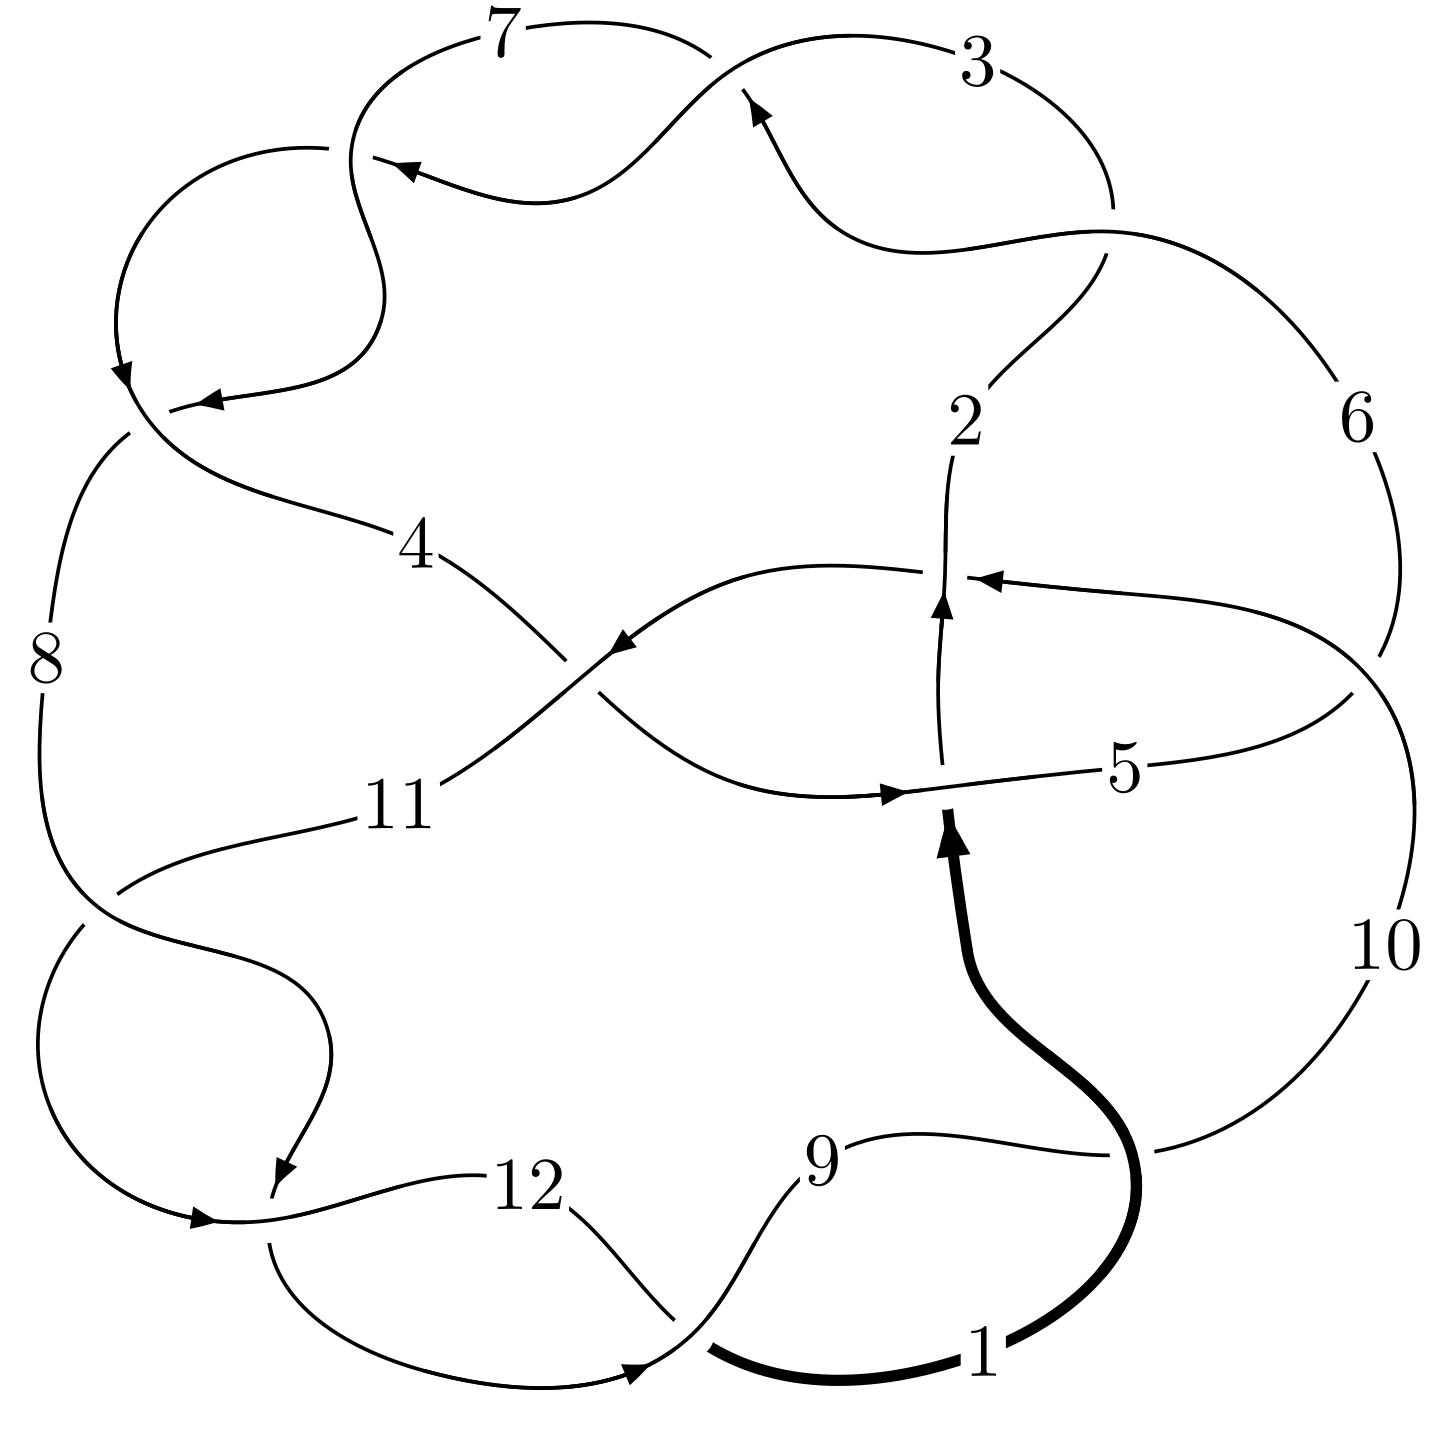
\includegraphics[width=112pt]{../../../GIT/diagram.site/Diagrams/png/2021_12a_1220.png}\\
\ \ \ A knot diagram\footnotemark}&
\allowdisplaybreaks
\textbf{Linearized knot diagam} \\
\cline{2-2}
 &
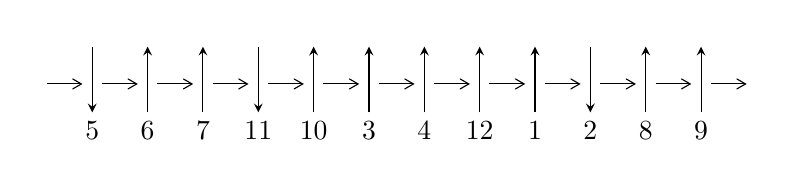
\begin{tikzpicture}[x=20pt, y=17pt]
	% nodes
	\node (C0) at (0, 0) {};
	\node (C1) at (1, 0) {};
	\node (C1U) at (1, +1) {};
	\node (C1D) at (1, -1) {5};

	\node (C2) at (2, 0) {};
	\node (C2U) at (2, +1) {};
	\node (C2D) at (2, -1) {6};

	\node (C3) at (3, 0) {};
	\node (C3U) at (3, +1) {};
	\node (C3D) at (3, -1) {7};

	\node (C4) at (4, 0) {};
	\node (C4U) at (4, +1) {};
	\node (C4D) at (4, -1) {11};

	\node (C5) at (5, 0) {};
	\node (C5U) at (5, +1) {};
	\node (C5D) at (5, -1) {10};

	\node (C6) at (6, 0) {};
	\node (C6U) at (6, +1) {};
	\node (C6D) at (6, -1) {3};

	\node (C7) at (7, 0) {};
	\node (C7U) at (7, +1) {};
	\node (C7D) at (7, -1) {4};

	\node (C8) at (8, 0) {};
	\node (C8U) at (8, +1) {};
	\node (C8D) at (8, -1) {12};

	\node (C9) at (9, 0) {};
	\node (C9U) at (9, +1) {};
	\node (C9D) at (9, -1) {1};

	\node (C10) at (10, 0) {};
	\node (C10U) at (10, +1) {};
	\node (C10D) at (10, -1) {2};

	\node (C11) at (11, 0) {};
	\node (C11U) at (11, +1) {};
	\node (C11D) at (11, -1) {8};

	\node (C12) at (12, 0) {};
	\node (C12U) at (12, +1) {};
	\node (C12D) at (12, -1) {9};
	\node (C13) at (13, 0) {};

	% arrows
	\draw[->,>={angle 60}]
	(C0) edge (C1) (C1) edge (C2) (C2) edge (C3) (C3) edge (C4) (C4) edge (C5) (C5) edge (C6) (C6) edge (C7) (C7) edge (C8) (C8) edge (C9) (C9) edge (C10) (C10) edge (C11) (C11) edge (C12) (C12) edge (C13) ;	\draw[->,>=stealth]
	(C1U) edge (C1D) (C2D) edge (C2U) (C3D) edge (C3U) (C4U) edge (C4D) (C5D) edge (C5U) (C6D) edge (C6U) (C7D) edge (C7U) (C8D) edge (C8U) (C9D) edge (C9U) (C10U) edge (C10D) (C11D) edge (C11U) (C12D) edge (C12U) ;
	\end{tikzpicture} \\
\hhline{~~} \\& 
\textbf{Solving Sequence} \\ \cline{2-2} 
 &
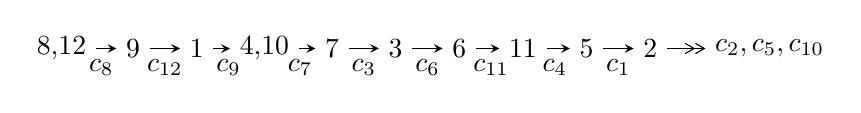
\begin{tikzpicture}[x=23pt, y=7pt]
	% node
	\node (A0) at (-1/8, 0) {8,12};
	\node (A1) at (1, 0) {9};
	\node (A2) at (2, 0) {1};
	\node (A3) at (49/16, 0) {4,10};
	\node (A4) at (33/8, 0) {7};
	\node (A5) at (41/8, 0) {3};
	\node (A6) at (49/8, 0) {6};
	\node (A7) at (57/8, 0) {11};
	\node (A8) at (65/8, 0) {5};
	\node (A9) at (73/8, 0) {2};
	\node (C1) at (1/2, -1) {$c_{8}$};
	\node (C2) at (3/2, -1) {$c_{12}$};
	\node (C3) at (5/2, -1) {$c_{9}$};
	\node (C4) at (29/8, -1) {$c_{7}$};
	\node (C5) at (37/8, -1) {$c_{3}$};
	\node (C6) at (45/8, -1) {$c_{6}$};
	\node (C7) at (53/8, -1) {$c_{11}$};
	\node (C8) at (61/8, -1) {$c_{4}$};
	\node (C9) at (69/8, -1) {$c_{1}$};
	\node (A10) at (11, 0) {$c_{2},c_{5},c_{10}$};

	% edge
	\draw[->,>=stealth]	
	(A0) edge (A1) (A1) edge (A2) (A2) edge (A3) (A3) edge (A4) (A4) edge (A5) (A5) edge (A6) (A6) edge (A7) (A7) edge (A8) (A8) edge (A9) ;
	\draw[->>,>={angle 60}]	
	(A9) edge (A10);
\end{tikzpicture} \\ 

\end{tabular} \\

\footnotetext{
The image of knot diagram is generated by the software ``\textbf{Draw programme}" developed by Andrew Bartholomew(\url{http://www.layer8.co.uk/maths/draw/index.htm\#Running-draw}), where we modified some parts for our purpose(\url{https://github.com/CATsTAILs/LinksPainter}).
}\phantom \\ \newline 
\centering \textbf{Ideals for irreducible components\footnotemark of $X_{\text{par}}$} 
 
\begin{align*}
I^u_{1}&=\langle 
b+u,\;-2 u^8-3 u^7+9 u^6+11 u^5-14 u^4-8 u^3+11 u^2+a+2,\\
\phantom{I^u_{1}}&\phantom{= \langle  }u^9+2 u^8-4 u^7-8 u^6+5 u^5+8 u^4-4 u^3-3 u^2- u-1\rangle \\
I^u_{2}&=\langle 
-2.05889\times10^{21} u^{39}-4.20027\times10^{20} u^{38}+\cdots+5.82584\times10^{21} b+1.03593\times10^{20},\\
\phantom{I^u_{2}}&\phantom{= \langle  }2.35540\times10^{21} u^{39}+3.66482\times10^{21} u^{38}+\cdots+2.91292\times10^{21} a+2.62000\times10^{21},\;u^{40}+2 u^{39}+\cdots+11 u+1\rangle \\
I^u_{3}&=\langle 
b-1,\;a+2,\;u^2- u-1\rangle \\
I^u_{4}&=\langle 
2 b+a,\;a^2-2 a-4,\;u+1\rangle \\
\\
\end{align*}
\raggedright * 4 irreducible components of $\dim_{\mathbb{C}}=0$, with total 53 representations.\\
\footnotetext{All coefficients of polynomials are rational numbers. But the coefficients are sometimes approximated in decimal forms when there is not enough margin.}
\newpage
\renewcommand{\arraystretch}{1}
\centering \section*{I. $I^u_{1}= \langle b+u,\;-2 u^8-3 u^7+\cdots+a+2,\;u^9+2 u^8+\cdots- u-1 \rangle$}
\flushleft \textbf{(i) Arc colorings}\\
\begin{tabular}{m{7pt} m{180pt} m{7pt} m{180pt} }
\flushright $a_{8}=$&$\begin{pmatrix}1\\0\end{pmatrix}$ \\
\flushright $a_{12}=$&$\begin{pmatrix}0\\u\end{pmatrix}$ \\
\flushright $a_{9}=$&$\begin{pmatrix}1\\- u^2\end{pmatrix}$ \\
\flushright $a_{1}=$&$\begin{pmatrix}u\\- u^3+u\end{pmatrix}$ \\
\flushright $a_{4}=$&$\begin{pmatrix}2 u^8+3 u^7-9 u^6-11 u^5+14 u^4+8 u^3-11 u^2-2\\- u\end{pmatrix}$ \\
\flushright $a_{10}=$&$\begin{pmatrix}- u^2+1\\u^4-2 u^2\end{pmatrix}$ \\
\flushright $a_{7}=$&$\begin{pmatrix}u^8+u^7-5 u^6-4 u^5+8 u^4+3 u^3-6 u^2-1\\u^2\end{pmatrix}$ \\
\flushright $a_{3}=$&$\begin{pmatrix}u^8+2 u^7-5 u^6-8 u^5+9 u^4+6 u^3-8 u^2-1\\u^3- u\end{pmatrix}$ \\
\flushright $a_{6}=$&$\begin{pmatrix}u^8+2 u^7-5 u^6-8 u^5+10 u^4+7 u^3-9 u^2-2\\- u^4+2 u^2\end{pmatrix}$ \\
\flushright $a_{11}=$&$\begin{pmatrix}- u\\u\end{pmatrix}$ \\
\flushright $a_{5}=$&$\begin{pmatrix}u^8+2 u^7-5 u^6-8 u^5+9 u^4+7 u^3-8 u^2- u-1\\u^8+u^7-4 u^6-3 u^5+5 u^4+u^3-3 u^2-1\end{pmatrix}$ \\
\flushright $a_{2}=$&$\begin{pmatrix}- u^8- u^7+5 u^6+3 u^5-8 u^4- u^3+5 u^2+u\\u^5-3 u^3+u\end{pmatrix}$\\&\end{tabular}
\flushleft \textbf{(ii) Obstruction class $= -1$}\\~\\
\flushleft \textbf{(iii) Cusp Shapes $= 16 u^8+24 u^7-76 u^6-84 u^5+124 u^4+40 u^3-88 u^2+20 u-22$}\\~\\
\newpage\renewcommand{\arraystretch}{1}
\flushleft \textbf{(iv) u-Polynomials at the component}\newline \\
\begin{tabular}{m{50pt}|m{274pt}}
Crossings & \hspace{64pt}u-Polynomials at each crossing \\
\hline $$\begin{aligned}c_{1},c_{10}\end{aligned}$$&$\begin{aligned}
&u^9-2 u^6+5 u^5-2 u^4-4 u^3-3 u^2+3 u+1
\end{aligned}$\\
\hline $$\begin{aligned}c_{2},c_{3},c_{6}\\c_{7},c_{8},c_{9}\\c_{11},c_{12}\end{aligned}$$&$\begin{aligned}
&u^9-2 u^8-4 u^7+8 u^6+5 u^5-8 u^4-4 u^3+3 u^2- u+1
\end{aligned}$\\
\hline $$\begin{aligned}c_{4}\end{aligned}$$&$\begin{aligned}
&u^9+13 u^8+\cdots+320 u+64
\end{aligned}$\\
\hline $$\begin{aligned}c_{5}\end{aligned}$$&$\begin{aligned}
&u^9+13 u^8+71 u^7+214 u^6+390 u^5+435 u^4+279 u^3+78 u^2-8 u-8
\end{aligned}$\\
\hline
\end{tabular}\\~\\
\newpage\renewcommand{\arraystretch}{1}
\flushleft \textbf{(v) Riley Polynomials at the component}\newline \\
\begin{tabular}{m{50pt}|m{274pt}}
Crossings & \hspace{64pt}Riley Polynomials at each crossing \\
\hline $$\begin{aligned}c_{1},c_{10}\end{aligned}$$&$\begin{aligned}
&y^9+10 y^7-12 y^6+23 y^5-56 y^4+38 y^3-29 y^2+15 y-1
\end{aligned}$\\
\hline $$\begin{aligned}c_{2},c_{3},c_{6}\\c_{7},c_{8},c_{9}\\c_{11},c_{12}\end{aligned}$$&$\begin{aligned}
&y^9-12 y^8+58 y^7-144 y^6+195 y^5-140 y^4+38 y^3+15 y^2-5 y-1
\end{aligned}$\\
\hline $$\begin{aligned}c_{4}\end{aligned}$$&$\begin{aligned}
&y^9-21 y^8+\cdots+8192 y-4096
\end{aligned}$\\
\hline $$\begin{aligned}c_{5}\end{aligned}$$&$\begin{aligned}
&y^9-27 y^8+\cdots+1312 y-64
\end{aligned}$\\
\hline
\end{tabular}\\~\\
\newpage\flushleft \textbf{(vi) Complex Volumes and Cusp Shapes}
$$\begin{array}{c|c|c}  
\text{Solutions to }I^u_{1}& \I (\text{vol} + \sqrt{-1}CS) & \text{Cusp shape}\\
 \hline 
\begin{aligned}
u &= \phantom{-}0.927341 + 0.453196 I \\
a &= \phantom{-}0.991720 - 0.824614 I \\
b &= -0.927341 - 0.453196 I\end{aligned}
 & \phantom{-}4.81531 + 7.88365 I & \phantom{-}13.1197 - 8.5237 I \\ \hline\begin{aligned}
u &= \phantom{-}0.927341 - 0.453196 I \\
a &= \phantom{-}0.991720 + 0.824614 I \\
b &= -0.927341 + 0.453196 I\end{aligned}
 & \phantom{-}4.81531 - 7.88365 I & \phantom{-}13.1197 + 8.5237 I \\ \hline\begin{aligned}
u &= -0.659939\phantom{ +0.000000I} \\
a &= -5.89270\phantom{ +0.000000I} \\
b &= \phantom{-}0.659939\phantom{ +0.000000I}\end{aligned}
 & \phantom{-}2.11613\phantom{ +0.000000I} & -57.9970\phantom{ +0.000000I} \\ \hline\begin{aligned}
u &= -1.43521\phantom{ +0.000000I} \\
a &= -2.20604\phantom{ +0.000000I} \\
b &= \phantom{-}1.43521\phantom{ +0.000000I}\end{aligned}
 & \phantom{-}8.30534\phantom{ +0.000000I} & \phantom{-}10.1970\phantom{ +0.000000I} \\ \hline\begin{aligned}
u &= \phantom{-}0.002669 + 0.448114 I \\
a &= \phantom{-}0.830042 - 0.971880 I \\
b &= -0.002669 - 0.448114 I\end{aligned}
 & -0.78700 - 1.41074 I & \phantom{-}1.25059 + 3.40619 I \\ \hline\begin{aligned}
u &= \phantom{-}0.002669 - 0.448114 I \\
a &= \phantom{-}0.830042 + 0.971880 I \\
b &= -0.002669 + 0.448114 I\end{aligned}
 & -0.78700 + 1.41074 I & \phantom{-}1.25059 - 3.40619 I \\ \hline\begin{aligned}
u &= \phantom{-}1.66419\phantom{ +0.000000I} \\
a &= \phantom{-}3.91567\phantom{ +0.000000I} \\
b &= -1.66419\phantom{ +0.000000I}\end{aligned}
 & \phantom{-}18.8023\phantom{ +0.000000I} & \phantom{-}6.12260\phantom{ +0.000000I} \\ \hline\begin{aligned}
u &= -1.71453 + 0.16075 I \\
a &= -2.23022 - 0.99164 I \\
b &= \phantom{-}1.71453 - 0.16075 I\end{aligned}
 & -16.1728 - 13.0673 I & \phantom{-}15.4687 + 5.5944 I \\ \hline\begin{aligned}
u &= -1.71453 - 0.16075 I \\
a &= -2.23022 + 0.99164 I \\
b &= \phantom{-}1.71453 + 0.16075 I\end{aligned}
 & -16.1728 + 13.0673 I & \phantom{-}15.4687 - 5.5944 I\\
 \hline 
 \end{array}$$\newpage\newpage\renewcommand{\arraystretch}{1}
\centering \section*{II. $I^u_{2}= \langle -2.06\times10^{21} u^{39}-4.20\times10^{20} u^{38}+\cdots+5.83\times10^{21} b+1.04\times10^{20},\;2.36\times10^{21} u^{39}+3.66\times10^{21} u^{38}+\cdots+2.91\times10^{21} a+2.62\times10^{21},\;u^{40}+2 u^{39}+\cdots+11 u+1 \rangle$}
\flushleft \textbf{(i) Arc colorings}\\
\begin{tabular}{m{7pt} m{180pt} m{7pt} m{180pt} }
\flushright $a_{8}=$&$\begin{pmatrix}1\\0\end{pmatrix}$ \\
\flushright $a_{12}=$&$\begin{pmatrix}0\\u\end{pmatrix}$ \\
\flushright $a_{9}=$&$\begin{pmatrix}1\\- u^2\end{pmatrix}$ \\
\flushright $a_{1}=$&$\begin{pmatrix}u\\- u^3+u\end{pmatrix}$ \\
\flushright $a_{4}=$&$\begin{pmatrix}-0.808605 u^{39}-1.25813 u^{38}+\cdots-36.2164 u-0.899441\\0.353407 u^{39}+0.0720972 u^{38}+\cdots-5.91849 u-0.0177816\end{pmatrix}$ \\
\flushright $a_{10}=$&$\begin{pmatrix}- u^2+1\\u^4-2 u^2\end{pmatrix}$ \\
\flushright $a_{7}=$&$\begin{pmatrix}-2.15713 u^{39}-2.78559 u^{38}+\cdots-51.4085 u-3.21686\\1.21823 u^{39}+1.13143 u^{38}+\cdots+2.86886 u+0.489002\end{pmatrix}$ \\
\flushright $a_{3}=$&$\begin{pmatrix}-0.342472 u^{39}-0.586708 u^{38}+\cdots-13.6913 u+0.476673\\-0.105307 u^{39}+0.107577 u^{38}+\cdots+3.48164 u+0.766785\end{pmatrix}$ \\
\flushright $a_{6}=$&$\begin{pmatrix}-1.72446 u^{39}-2.57322 u^{38}+\cdots-46.0801 u-1.47304\\0.444440 u^{39}+0.320947 u^{38}+\cdots-9.97662 u-0.424757\end{pmatrix}$ \\
\flushright $a_{11}=$&$\begin{pmatrix}- u\\u\end{pmatrix}$ \\
\flushright $a_{5}=$&$\begin{pmatrix}-2.06730 u^{39}-2.12671 u^{38}+\cdots-39.7036 u-1.17508\\1.61210 u^{39}+0.940683 u^{38}+\cdots-2.43132 u+0.257852\end{pmatrix}$ \\
\flushright $a_{2}=$&$\begin{pmatrix}-3.62228 u^{39}-3.22253 u^{38}+\cdots-46.8489 u-5.52801\\3.45055 u^{39}+2.41041 u^{38}+\cdots+6.30294 u+0.399746\end{pmatrix}$\\&\end{tabular}
\flushleft \textbf{(ii) Obstruction class $= -1$}\\~\\
\flushleft \textbf{(iii) Cusp Shapes $= -\frac{2825773251700395997919}{728229534914329869523} u^{39}-\frac{2538801677611388911625}{728229534914329869523} u^{38}+\cdots-\frac{40264361670734015524833}{728229534914329869523} u+\frac{2631129163027084440997}{728229534914329869523}$}\\~\\
\newpage\renewcommand{\arraystretch}{1}
\flushleft \textbf{(iv) u-Polynomials at the component}\newline \\
\begin{tabular}{m{50pt}|m{274pt}}
Crossings & \hspace{64pt}u-Polynomials at each crossing \\
\hline $$\begin{aligned}c_{1},c_{10}\end{aligned}$$&$\begin{aligned}
&u^{40}+3 u^{39}+\cdots+11 u^2+4
\end{aligned}$\\
\hline $$\begin{aligned}c_{2},c_{3},c_{6}\\c_{7},c_{8},c_{9}\\c_{11},c_{12}\end{aligned}$$&$\begin{aligned}
&u^{40}-2 u^{39}+\cdots-11 u+1
\end{aligned}$\\
\hline $$\begin{aligned}c_{4}\end{aligned}$$&$\begin{aligned}
&(u^{20}-7 u^{19}+\cdots-191 u+47)^{2}
\end{aligned}$\\
\hline $$\begin{aligned}c_{5}\end{aligned}$$&$\begin{aligned}
&(u^{20}-6 u^{19}+\cdots-16 u+1)^{2}
\end{aligned}$\\
\hline
\end{tabular}\\~\\
\newpage\renewcommand{\arraystretch}{1}
\flushleft \textbf{(v) Riley Polynomials at the component}\newline \\
\begin{tabular}{m{50pt}|m{274pt}}
Crossings & \hspace{64pt}Riley Polynomials at each crossing \\
\hline $$\begin{aligned}c_{1},c_{10}\end{aligned}$$&$\begin{aligned}
&y^{40}+13 y^{39}+\cdots+88 y+16
\end{aligned}$\\
\hline $$\begin{aligned}c_{2},c_{3},c_{6}\\c_{7},c_{8},c_{9}\\c_{11},c_{12}\end{aligned}$$&$\begin{aligned}
&y^{40}-50 y^{39}+\cdots-49 y+1
\end{aligned}$\\
\hline $$\begin{aligned}c_{4}\end{aligned}$$&$\begin{aligned}
&(y^{20}+3 y^{19}+\cdots+16629 y+2209)^{2}
\end{aligned}$\\
\hline $$\begin{aligned}c_{5}\end{aligned}$$&$\begin{aligned}
&(y^{20}-24 y^{19}+\cdots-210 y+1)^{2}
\end{aligned}$\\
\hline
\end{tabular}\\~\\
\newpage\flushleft \textbf{(vi) Complex Volumes and Cusp Shapes}
$$\begin{array}{c|c|c}  
\text{Solutions to }I^u_{2}& \I (\text{vol} + \sqrt{-1}CS) & \text{Cusp shape}\\
 \hline 
\begin{aligned}
u &= \phantom{-}0.964193 + 0.183114 I \\
a &= \phantom{-}1.81237 - 1.07233 I \\
b &= -1.68373 - 0.13054 I\end{aligned}
 & \phantom{-}12.94220 + 2.92572 I & \phantom{-}16.8415 - 2.9709 I \\ \hline\begin{aligned}
u &= \phantom{-}0.964193 - 0.183114 I \\
a &= \phantom{-}1.81237 + 1.07233 I \\
b &= -1.68373 + 0.13054 I\end{aligned}
 & \phantom{-}12.94220 - 2.92572 I & \phantom{-}16.8415 + 2.9709 I \\ \hline\begin{aligned}
u &= -0.871135 + 0.550509 I \\
a &= \phantom{-}0.457497 + 0.668616 I \\
b &= -0.858752 - 0.047670 I\end{aligned}
 & \phantom{-}4.04379 - 0.34594 I & \phantom{-}19.0261 - 0.3312 I \\ \hline\begin{aligned}
u &= -0.871135 - 0.550509 I \\
a &= \phantom{-}0.457497 - 0.668616 I \\
b &= -0.858752 + 0.047670 I\end{aligned}
 & \phantom{-}4.04379 + 0.34594 I & \phantom{-}19.0261 + 0.3312 I \\ \hline\begin{aligned}
u &= -0.094224 + 0.891903 I \\
a &= -0.324167 - 0.354300 I \\
b &= \phantom{-}1.67359 - 0.07029 I\end{aligned}
 & \phantom{-}10.57610 - 5.30216 I & \phantom{-}12.68744 + 4.85316 I \\ \hline\begin{aligned}
u &= -0.094224 - 0.891903 I \\
a &= -0.324167 + 0.354300 I \\
b &= \phantom{-}1.67359 + 0.07029 I\end{aligned}
 & \phantom{-}10.57610 + 5.30216 I & \phantom{-}12.68744 - 4.85316 I \\ \hline\begin{aligned}
u &= \phantom{-}0.841679 + 0.285962 I \\
a &= -0.249728 + 0.281271 I \\
b &= \phantom{-}0.079408 + 0.721551 I\end{aligned}
 & \phantom{-}1.73170 + 3.96676 I & \phantom{-}10.64355 - 7.18805 I \\ \hline\begin{aligned}
u &= \phantom{-}0.841679 - 0.285962 I \\
a &= -0.249728 - 0.281271 I \\
b &= \phantom{-}0.079408 - 0.721551 I\end{aligned}
 & \phantom{-}1.73170 - 3.96676 I & \phantom{-}10.64355 + 7.18805 I \\ \hline\begin{aligned}
u &= \phantom{-}0.858752 + 0.047670 I \\
a &= -0.911277 - 0.334390 I \\
b &= \phantom{-}0.871135 - 0.550509 I\end{aligned}
 & \phantom{-}4.04379 - 0.34594 I & \phantom{-}19.0261 - 0.3312 I \\ \hline\begin{aligned}
u &= \phantom{-}0.858752 - 0.047670 I \\
a &= -0.911277 + 0.334390 I \\
b &= \phantom{-}0.871135 + 0.550509 I\end{aligned}
 & \phantom{-}4.04379 + 0.34594 I & \phantom{-}19.0261 + 0.3312 I\\
 \hline 
 \end{array}$$\newpage$$\begin{array}{c|c|c}  
\text{Solutions to }I^u_{2}& \I (\text{vol} + \sqrt{-1}CS) & \text{Cusp shape}\\
 \hline 
\begin{aligned}
u &= \phantom{-}0.996751 + 0.567865 I \\
a &= -1.56536 + 1.35978 I \\
b &= \phantom{-}1.69022 + 0.12129 I\end{aligned}
 & \phantom{-}13.9204 + 10.1318 I & \phantom{-}14.3223 - 6.7026 I \\ \hline\begin{aligned}
u &= \phantom{-}0.996751 - 0.567865 I \\
a &= -1.56536 - 1.35978 I \\
b &= \phantom{-}1.69022 - 0.12129 I\end{aligned}
 & \phantom{-}13.9204 - 10.1318 I & \phantom{-}14.3223 + 6.7026 I \\ \hline\begin{aligned}
u &= -1.15373\phantom{ +0.000000I} \\
a &= \phantom{-}0.932910\phantom{ +0.000000I} \\
b &= -0.386843\phantom{ +0.000000I}\end{aligned}
 & \phantom{-}2.16630\phantom{ +0.000000I} & -1.22340\phantom{ +0.000000I} \\ \hline\begin{aligned}
u &= -0.952961 + 0.719204 I \\
a &= -1.31275 - 0.94519 I \\
b &= \phantom{-}1.68108 + 0.01576 I\end{aligned}
 & \phantom{-}13.06170 - 0.07749 I & \phantom{-}17.5894 + 0. I\phantom{ +0.000000I} \\ \hline\begin{aligned}
u &= -0.952961 - 0.719204 I \\
a &= -1.31275 + 0.94519 I \\
b &= \phantom{-}1.68108 - 0.01576 I\end{aligned}
 & \phantom{-}13.06170 + 0.07749 I & \phantom{-}17.5894 + 0. I\phantom{ +0.000000I} \\ \hline\begin{aligned}
u &= -0.745297\phantom{ +0.000000I} \\
a &= \phantom{-}6.94927\phantom{ +0.000000I} \\
b &= -1.62727\phantom{ +0.000000I}\end{aligned}
 & \phantom{-}10.1903\phantom{ +0.000000I} & -24.0970\phantom{ +0.000000I} \\ \hline\begin{aligned}
u &= -0.079408 + 0.721551 I \\
a &= -0.182590 + 0.422871 I \\
b &= -0.841679 + 0.285962 I\end{aligned}
 & \phantom{-}1.73170 - 3.96676 I & \phantom{-}10.64355 + 7.18805 I \\ \hline\begin{aligned}
u &= -0.079408 - 0.721551 I \\
a &= -0.182590 - 0.422871 I \\
b &= -0.841679 - 0.285962 I\end{aligned}
 & \phantom{-}1.73170 + 3.96676 I & \phantom{-}10.64355 - 7.18805 I \\ \hline\begin{aligned}
u &= -0.651290 + 0.157168 I \\
a &= \phantom{-}0.836528 - 0.648564 I \\
b &= \phantom{-}0.154389 - 0.087035 I\end{aligned}
 & \phantom{-}1.239960 - 0.397086 I & \phantom{-}8.64524 + 0.31446 I \\ \hline\begin{aligned}
u &= -0.651290 - 0.157168 I \\
a &= \phantom{-}0.836528 + 0.648564 I \\
b &= \phantom{-}0.154389 + 0.087035 I\end{aligned}
 & \phantom{-}1.239960 + 0.397086 I & \phantom{-}8.64524 - 0.31446 I\\
 \hline 
 \end{array}$$\newpage$$\begin{array}{c|c|c}  
\text{Solutions to }I^u_{2}& \I (\text{vol} + \sqrt{-1}CS) & \text{Cusp shape}\\
 \hline 
\begin{aligned}
u &= -0.224632 + 0.357420 I \\
a &= -2.05994 + 0.87263 I \\
b &= -1.63217 + 0.03725 I\end{aligned}
 & \phantom{-}9.29517 - 1.07904 I & \phantom{-}8.55163 - 1.79539 I \\ \hline\begin{aligned}
u &= -0.224632 - 0.357420 I \\
a &= -2.05994 - 0.87263 I \\
b &= -1.63217 - 0.03725 I\end{aligned}
 & \phantom{-}9.29517 + 1.07904 I & \phantom{-}8.55163 + 1.79539 I \\ \hline\begin{aligned}
u &= \phantom{-}0.386843\phantom{ +0.000000I} \\
a &= -2.78232\phantom{ +0.000000I} \\
b &= \phantom{-}1.15373\phantom{ +0.000000I}\end{aligned}
 & \phantom{-}2.16630\phantom{ +0.000000I} & -1.22340\phantom{ +0.000000I} \\ \hline\begin{aligned}
u &= \phantom{-}1.62727\phantom{ +0.000000I} \\
a &= -3.18279\phantom{ +0.000000I} \\
b &= \phantom{-}0.745297\phantom{ +0.000000I}\end{aligned}
 & \phantom{-}10.1903\phantom{ +0.000000I} & \phantom{-0.000000 } 0 \\ \hline\begin{aligned}
u &= \phantom{-}1.63217 + 0.03725 I \\
a &= \phantom{-}0.105394 + 0.568790 I \\
b &= \phantom{-}0.224632 + 0.357420 I\end{aligned}
 & \phantom{-}9.29517 + 1.07904 I & \phantom{-0.000000 } 0 \\ \hline\begin{aligned}
u &= \phantom{-}1.63217 - 0.03725 I \\
a &= \phantom{-}0.105394 - 0.568790 I \\
b &= \phantom{-}0.224632 - 0.357420 I\end{aligned}
 & \phantom{-}9.29517 - 1.07904 I & \phantom{-0.000000 } 0 \\ \hline\begin{aligned}
u &= -1.67359 + 0.07029 I \\
a &= -0.213109 + 0.143861 I \\
b &= \phantom{-}0.094224 - 0.891903 I\end{aligned}
 & \phantom{-}10.57610 - 5.30216 I & \phantom{-0.000000 } 0 \\ \hline\begin{aligned}
u &= -1.67359 - 0.07029 I \\
a &= -0.213109 - 0.143861 I \\
b &= \phantom{-}0.094224 + 0.891903 I\end{aligned}
 & \phantom{-}10.57610 + 5.30216 I & \phantom{-0.000000 } 0 \\ \hline\begin{aligned}
u &= -1.68108 + 0.01576 I \\
a &= -1.148200 - 0.036582 I \\
b &= \phantom{-}0.952961 + 0.719204 I\end{aligned}
 & \phantom{-}13.06170 + 0.07749 I & \phantom{-0.000000 } 0 \\ \hline\begin{aligned}
u &= -1.68108 - 0.01576 I \\
a &= -1.148200 + 0.036582 I \\
b &= \phantom{-}0.952961 - 0.719204 I\end{aligned}
 & \phantom{-}13.06170 - 0.07749 I & \phantom{-0.000000 } 0\\
 \hline 
 \end{array}$$\newpage$$\begin{array}{c|c|c}  
\text{Solutions to }I^u_{2}& \I (\text{vol} + \sqrt{-1}CS) & \text{Cusp shape}\\
 \hline 
\begin{aligned}
u &= \phantom{-}1.68373 + 0.13054 I \\
a &= \phantom{-}1.115450 - 0.503449 I \\
b &= -0.964193 - 0.183114 I\end{aligned}
 & \phantom{-}12.94220 + 2.92572 I & \phantom{-0.000000 } 0 \\ \hline\begin{aligned}
u &= \phantom{-}1.68373 - 0.13054 I \\
a &= \phantom{-}1.115450 + 0.503449 I \\
b &= -0.964193 + 0.183114 I\end{aligned}
 & \phantom{-}12.94220 - 2.92572 I & \phantom{-0.000000 } 0 \\ \hline\begin{aligned}
u &= -1.69022 + 0.12129 I \\
a &= \phantom{-}1.353200 + 0.373072 I \\
b &= -0.996751 + 0.567865 I\end{aligned}
 & \phantom{-}13.9204 - 10.1318 I & \phantom{-0.000000 } 0 \\ \hline\begin{aligned}
u &= -1.69022 - 0.12129 I \\
a &= \phantom{-}1.353200 - 0.373072 I \\
b &= -0.996751 - 0.567865 I\end{aligned}
 & \phantom{-}13.9204 + 10.1318 I & \phantom{-0.000000 } 0 \\ \hline\begin{aligned}
u &= -1.70429 + 0.04276 I \\
a &= \phantom{-}2.28176 + 0.53396 I \\
b &= -1.74240 + 0.19593 I\end{aligned}
 & -17.0616 - 3.7959 I & \phantom{-0.000000 } 0 \\ \hline\begin{aligned}
u &= -1.70429 - 0.04276 I \\
a &= \phantom{-}2.28176 - 0.53396 I \\
b &= -1.74240 - 0.19593 I\end{aligned}
 & -17.0616 + 3.7959 I & \phantom{-0.000000 } 0 \\ \hline\begin{aligned}
u &= \phantom{-}1.74240 + 0.19593 I \\
a &= -2.16516 + 0.70975 I \\
b &= \phantom{-}1.70429 + 0.04276 I\end{aligned}
 & -17.0616 + 3.7959 I & \phantom{-0.000000 } 0 \\ \hline\begin{aligned}
u &= \phantom{-}1.74240 - 0.19593 I \\
a &= -2.16516 - 0.70975 I \\
b &= \phantom{-}1.70429 - 0.04276 I\end{aligned}
 & -17.0616 - 3.7959 I & \phantom{-0.000000 } 0 \\ \hline\begin{aligned}
u &= -0.154389 + 0.087035 I \\
a &= \phantom{-}3.71156 - 1.49520 I \\
b &= \phantom{-}0.651290 - 0.157168 I\end{aligned}
 & \phantom{-}1.239960 - 0.397086 I & \phantom{-}8.64524 + 0.31446 I \\ \hline\begin{aligned}
u &= -0.154389 - 0.087035 I \\
a &= \phantom{-}3.71156 + 1.49520 I \\
b &= \phantom{-}0.651290 + 0.157168 I\end{aligned}
 & \phantom{-}1.239960 + 0.397086 I & \phantom{-}8.64524 - 0.31446 I\\
 \hline 
 \end{array}$$\newpage\newpage\renewcommand{\arraystretch}{1}
\centering \section*{III. $I^u_{3}= \langle b-1,\;a+2,\;u^2- u-1 \rangle$}
\flushleft \textbf{(i) Arc colorings}\\
\begin{tabular}{m{7pt} m{180pt} m{7pt} m{180pt} }
\flushright $a_{8}=$&$\begin{pmatrix}1\\0\end{pmatrix}$ \\
\flushright $a_{12}=$&$\begin{pmatrix}0\\u\end{pmatrix}$ \\
\flushright $a_{9}=$&$\begin{pmatrix}1\\- u-1\end{pmatrix}$ \\
\flushright $a_{1}=$&$\begin{pmatrix}u\\- u-1\end{pmatrix}$ \\
\flushright $a_{4}=$&$\begin{pmatrix}-2\\1\end{pmatrix}$ \\
\flushright $a_{10}=$&$\begin{pmatrix}- u\\u\end{pmatrix}$ \\
\flushright $a_{7}=$&$\begin{pmatrix}-1\\1\end{pmatrix}$ \\
\flushright $a_{3}=$&$\begin{pmatrix}-1\\0\end{pmatrix}$ \\
\flushright $a_{6}=$&$\begin{pmatrix}-2\\1\end{pmatrix}$ \\
\flushright $a_{11}=$&$\begin{pmatrix}- u\\u\end{pmatrix}$ \\
\flushright $a_{5}=$&$\begin{pmatrix}u-1\\- u\end{pmatrix}$ \\
\flushright $a_{2}=$&$\begin{pmatrix}1\\-1\end{pmatrix}$\\&\end{tabular}
\flushleft \textbf{(ii) Obstruction class $= 1$}\\~\\
\flushleft \textbf{(iii) Cusp Shapes $= 17$}\\~\\
\newpage\renewcommand{\arraystretch}{1}
\flushleft \textbf{(iv) u-Polynomials at the component}\newline \\
\begin{tabular}{m{50pt}|m{274pt}}
Crossings & \hspace{64pt}u-Polynomials at each crossing \\
\hline $$\begin{aligned}c_{1},c_{2},c_{3}\end{aligned}$$&$\begin{aligned}
&(u+1)^2
\end{aligned}$\\
\hline $$\begin{aligned}c_{4},c_{5},c_{11}\\c_{12}\end{aligned}$$&$\begin{aligned}
&u^2+u-1
\end{aligned}$\\
\hline $$\begin{aligned}c_{6},c_{7}\end{aligned}$$&$\begin{aligned}
&(u-1)^2
\end{aligned}$\\
\hline $$\begin{aligned}c_{8},c_{9}\end{aligned}$$&$\begin{aligned}
&u^2- u-1
\end{aligned}$\\
\hline $$\begin{aligned}c_{10}\end{aligned}$$&$\begin{aligned}
&u^2
\end{aligned}$\\
\hline
\end{tabular}\\~\\
\newpage\renewcommand{\arraystretch}{1}
\flushleft \textbf{(v) Riley Polynomials at the component}\newline \\
\begin{tabular}{m{50pt}|m{274pt}}
Crossings & \hspace{64pt}Riley Polynomials at each crossing \\
\hline $$\begin{aligned}c_{1},c_{2},c_{3}\\c_{6},c_{7}\end{aligned}$$&$\begin{aligned}
&(y-1)^2
\end{aligned}$\\
\hline $$\begin{aligned}c_{4},c_{5},c_{8}\\c_{9},c_{11},c_{12}\end{aligned}$$&$\begin{aligned}
&y^2-3 y+1
\end{aligned}$\\
\hline $$\begin{aligned}c_{10}\end{aligned}$$&$\begin{aligned}
&y^2
\end{aligned}$\\
\hline
\end{tabular}\\~\\
\newpage\flushleft \textbf{(vi) Complex Volumes and Cusp Shapes}
$$\begin{array}{c|c|c}  
\text{Solutions to }I^u_{3}& \I (\text{vol} + \sqrt{-1}CS) & \text{Cusp shape}\\
 \hline 
\begin{aligned}
u &= -0.618034\phantom{ +0.000000I} \\
a &= -2.00000\phantom{ +0.000000I} \\
b &= \phantom{-}1.00000\phantom{ +0.000000I}\end{aligned}
 & \phantom{-}2.63189\phantom{ +0.000000I} & \phantom{-}17.0000\phantom{ +0.000000I} \\ \hline\begin{aligned}
u &= \phantom{-}1.61803\phantom{ +0.000000I} \\
a &= -2.00000\phantom{ +0.000000I} \\
b &= \phantom{-}1.00000\phantom{ +0.000000I}\end{aligned}
 & \phantom{-}10.5276\phantom{ +0.000000I} & \phantom{-}17.0000\phantom{ +0.000000I}\\
 \hline 
 \end{array}$$\newpage\newpage\renewcommand{\arraystretch}{1}
\centering \section*{IV. $I^u_{4}= \langle 2 b+a,\;a^2-2 a-4,\;u+1 \rangle$}
\flushleft \textbf{(i) Arc colorings}\\
\begin{tabular}{m{7pt} m{180pt} m{7pt} m{180pt} }
\flushright $a_{8}=$&$\begin{pmatrix}1\\0\end{pmatrix}$ \\
\flushright $a_{12}=$&$\begin{pmatrix}0\\-1\end{pmatrix}$ \\
\flushright $a_{9}=$&$\begin{pmatrix}1\\-1\end{pmatrix}$ \\
\flushright $a_{1}=$&$\begin{pmatrix}-1\\0\end{pmatrix}$ \\
\flushright $a_{4}=$&$\begin{pmatrix}a\\-\frac{1}{2} a\end{pmatrix}$ \\
\flushright $a_{10}=$&$\begin{pmatrix}0\\-1\end{pmatrix}$ \\
\flushright $a_{7}=$&$\begin{pmatrix}- a-1\\\frac{1}{2} a+1\end{pmatrix}$ \\
\flushright $a_{3}=$&$\begin{pmatrix}-\frac{1}{2} a-2\\\frac{1}{2} a+1\end{pmatrix}$ \\
\flushright $a_{6}=$&$\begin{pmatrix}\frac{1}{2} a\\-\frac{1}{2} a\end{pmatrix}$ \\
\flushright $a_{11}=$&$\begin{pmatrix}1\\-1\end{pmatrix}$ \\
\flushright $a_{5}=$&$\begin{pmatrix}\frac{1}{2} a\\0\end{pmatrix}$ \\
\flushright $a_{2}=$&$\begin{pmatrix}-1\\0\end{pmatrix}$\\&\end{tabular}
\flushleft \textbf{(ii) Obstruction class $= 1$}\\~\\
\flushleft \textbf{(iii) Cusp Shapes $= 17$}\\~\\
\newpage\renewcommand{\arraystretch}{1}
\flushleft \textbf{(iv) u-Polynomials at the component}\newline \\
\begin{tabular}{m{50pt}|m{274pt}}
Crossings & \hspace{64pt}u-Polynomials at each crossing \\
\hline $$\begin{aligned}c_{1}\end{aligned}$$&$\begin{aligned}
&u^2
\end{aligned}$\\
\hline $$\begin{aligned}c_{2},c_{3}\end{aligned}$$&$\begin{aligned}
&u^2- u-1
\end{aligned}$\\
\hline $$\begin{aligned}c_{4},c_{5},c_{6}\\c_{7}\end{aligned}$$&$\begin{aligned}
&u^2+u-1
\end{aligned}$\\
\hline $$\begin{aligned}c_{8},c_{9},c_{10}\end{aligned}$$&$\begin{aligned}
&(u+1)^2
\end{aligned}$\\
\hline $$\begin{aligned}c_{11},c_{12}\end{aligned}$$&$\begin{aligned}
&(u-1)^2
\end{aligned}$\\
\hline
\end{tabular}\\~\\
\newpage\renewcommand{\arraystretch}{1}
\flushleft \textbf{(v) Riley Polynomials at the component}\newline \\
\begin{tabular}{m{50pt}|m{274pt}}
Crossings & \hspace{64pt}Riley Polynomials at each crossing \\
\hline $$\begin{aligned}c_{1}\end{aligned}$$&$\begin{aligned}
&y^2
\end{aligned}$\\
\hline $$\begin{aligned}c_{2},c_{3},c_{4}\\c_{5},c_{6},c_{7}\end{aligned}$$&$\begin{aligned}
&y^2-3 y+1
\end{aligned}$\\
\hline $$\begin{aligned}c_{8},c_{9},c_{10}\\c_{11},c_{12}\end{aligned}$$&$\begin{aligned}
&(y-1)^2
\end{aligned}$\\
\hline
\end{tabular}\\~\\
\newpage\flushleft \textbf{(vi) Complex Volumes and Cusp Shapes}
$$\begin{array}{c|c|c}  
\text{Solutions to }I^u_{4}& \I (\text{vol} + \sqrt{-1}CS) & \text{Cusp shape}\\
 \hline 
\begin{aligned}
u &= -1.00000\phantom{ +0.000000I} \\
a &= -1.23607\phantom{ +0.000000I} \\
b &= \phantom{-}0.618034\phantom{ +0.000000I}\end{aligned}
 & \phantom{-}2.63189\phantom{ +0.000000I} & \phantom{-}17.0000\phantom{ +0.000000I} \\ \hline\begin{aligned}
u &= -1.00000\phantom{ +0.000000I} \\
a &= \phantom{-}3.23607\phantom{ +0.000000I} \\
b &= -1.61803\phantom{ +0.000000I}\end{aligned}
 & \phantom{-}10.5276\phantom{ +0.000000I} & \phantom{-}17.0000\phantom{ +0.000000I}\\
 \hline 
 \end{array}$$\newpage
\newpage\renewcommand{\arraystretch}{1}
\centering \section*{ V. u-Polynomials}
\begin{tabular}{m{50pt}|m{274pt}}
Crossings & \hspace{64pt}u-Polynomials at each crossing \\
\hline $$\begin{aligned}c_{1},c_{10}\end{aligned}$$&$\begin{aligned}
&u^2(u+1)^2(u^9-2 u^6+5 u^5-2 u^4-4 u^3-3 u^2+3 u+1)\\
&\cdot(u^{40}+3 u^{39}+\cdots+11 u^2+4)
\end{aligned}$\\
\hline $$\begin{aligned}c_{2},c_{3},c_{8}\\c_{9}\end{aligned}$$&$\begin{aligned}
&(u+1)^2(u^2- u-1)\\
&\cdot(u^9-2 u^8-4 u^7+8 u^6+5 u^5-8 u^4-4 u^3+3 u^2- u+1)\\
&\cdot(u^{40}-2 u^{39}+\cdots-11 u+1)
\end{aligned}$\\
\hline $$\begin{aligned}c_{4}\end{aligned}$$&$\begin{aligned}
&((u^2+u-1)^2)(u^9+13 u^8+\cdots+320 u+64)\\
&\cdot(u^{20}-7 u^{19}+\cdots-191 u+47)^{2}
\end{aligned}$\\
\hline $$\begin{aligned}c_{5}\end{aligned}$$&$\begin{aligned}
&(u^2+u-1)^2\\
&\cdot(u^9+13 u^8+71 u^7+214 u^6+390 u^5+435 u^4+279 u^3+78 u^2-8 u-8)\\
&\cdot(u^{20}-6 u^{19}+\cdots-16 u+1)^{2}
\end{aligned}$\\
\hline $$\begin{aligned}c_{6},c_{7},c_{11}\\c_{12}\end{aligned}$$&$\begin{aligned}
&(u-1)^2(u^2+u-1)\\
&\cdot(u^9-2 u^8-4 u^7+8 u^6+5 u^5-8 u^4-4 u^3+3 u^2- u+1)\\
&\cdot(u^{40}-2 u^{39}+\cdots-11 u+1)
\end{aligned}$\\
\hline
\end{tabular}\newpage\renewcommand{\arraystretch}{1}
\centering \section*{ VI. Riley Polynomials}
\begin{tabular}{m{50pt}|m{274pt}}
Crossings & \hspace{64pt}Riley Polynomials at each crossing \\
\hline $$\begin{aligned}c_{1},c_{10}\end{aligned}$$&$\begin{aligned}
&y^2(y-1)^2(y^9+10 y^7+\cdots+15 y-1)\\
&\cdot(y^{40}+13 y^{39}+\cdots+88 y+16)
\end{aligned}$\\
\hline $$\begin{aligned}c_{2},c_{3},c_{6}\\c_{7},c_{8},c_{9}\\c_{11},c_{12}\end{aligned}$$&$\begin{aligned}
&(y-1)^2(y^2-3 y+1)\\
&\cdot(y^9-12 y^8+58 y^7-144 y^6+195 y^5-140 y^4+38 y^3+15 y^2-5 y-1)\\
&\cdot(y^{40}-50 y^{39}+\cdots-49 y+1)
\end{aligned}$\\
\hline $$\begin{aligned}c_{4}\end{aligned}$$&$\begin{aligned}
&((y^2-3 y+1)^2)(y^9-21 y^8+\cdots+8192 y-4096)\\
&\cdot(y^{20}+3 y^{19}+\cdots+16629 y+2209)^{2}
\end{aligned}$\\
\hline $$\begin{aligned}c_{5}\end{aligned}$$&$\begin{aligned}
&((y^2-3 y+1)^2)(y^9-27 y^8+\cdots+1312 y-64)\\
&\cdot(y^{20}-24 y^{19}+\cdots-210 y+1)^{2}
\end{aligned}$\\
\hline
\end{tabular}
\vskip 2pc
\end{document}